\documentclass[acmtog,anonymous,review]{acmart}
\acmSubmissionID{4321}

\usepackage{booktabs} % For formal tables

\newcommand{\final}{0}

\input{TOG/package}
\input{TOG/macros}
% Einstein
\newcommand{\energy}{E}
\newcommand{\mass}{m}
\newcommand{\lightspeed}{c}

% dart throwing
\newcommand{\domainsym}{\Omega}
\newcommand{\dimnumber}{d} % dimensionality of the sample space
% note it should be $k$-d not $k$-$d$ as here "d" is an acronym for the word "dimension," not a variable.

\newcommand{\samplesym}{s}
\newcommand{\sample}{\samplesym{}}
\newcommand{\samplesetsym}{\mathcal{S}}
\newcommand{\sampleset}{\samplesetsym{}}
\newcommand{\sampleprime}{\samplesym^{\prime}{}}
\newcommand{\dist}{d}
\newcommand{\conflictdist}{r}
\newcommand{\union}{\oplus}
\newcommand{\failure}{f}
\newcommand{\assign}{\leftarrow}

\newcommand{\sparseError}{E_{scene}}
\newcommand{\pt}{\mathbf{q}}
\newcommand{\rayo}{\mathbf{x}}
\newcommand{\rayd}{\mathbf{v}}
\newcommand{\intersectionFunc}{p}

\newcommand{\SpatialPt}{\mathbf{q}}

\newcommand{\sphereNum}{N}
\newcommand{\sphereID}{n}
\newcommand{\sphereRadius}{r}

\newcommand{\projectionMatrix}{\mathbf{M}}
\newcommand{\imgSpaceError}{E_{image}}

\newcommand{\finalError}{E}
\newcommand{\latency}{l}

\newcommand{\mlpLayerNum}{N_{m}}
\newcommand{\mlpChannelNum}{N_{c}}
\newcommand{\image}{I}
\newcommand{\imageFoveal}{I_{f}}
\newcommand{\imageMid}{I_{m}}
\newcommand{\imageFar}{I_{p}}

\newcommand{\mlpFunc}{C}

\newcommand{\norm}[1]{\left\lVert#1\right\rVert}


\newcommand{\argmin}{\operatornamewithlimits{argmin}}

\newcommand{\camDir}{\mathbf{R}}
\newcommand{\gazeDir}{\mathbf{\rayd_g}}
\input{TOG/graphicspath}
\acmJournal{TOG}
\acmYear{2021}
\acmVolume{36}
\acmNumber{4}
\acmArticle{1}
\acmMonth{7} % July
\acmDOI{}
\acmSubmissionID{0200}



% TOG prefers author-name bib system with square brackets
\citestyle{acmauthoryear}
%\setcitestyle{nosort,square} % nosort to allow for manual chronological ordering

\usepackage[ruled]{algorithm2e} % For algorithms
\renewcommand{\algorithmcfname}{ALGORITHM}
\SetAlFnt{\small}
\SetAlCapFnt{\small}
\SetAlCapNameFnt{\small}
\SetAlCapHSkip{0pt}

% Metadata Information
\acmJournal{TOG}

% Document starts
\begin{document}
% Title portion
\title{Representing Scenes as Light Fields for Real Time Rendering in Virtual Reality Display}
% Representing Scenes as Neural Radiance Fields for View Synthesis

\begin{abstract}
Writing papers and managing projects are essential for conducting research.
A research paper describes the final outcomes, but can also help manage intermediate progress.
This document provides a template for writing papers and describes how to manage projects via drafts.

Start the abstract when you have some rough ideas, before they are forgotten amid your busy lives.
It does not need to be fancy, as long as you can understand your own writing later.
The eventual abstract should be the minimalist version of the entire paper, with key information outlined in the introduction.
\end{abstract}

%
% The code below should be generated by the tool at
% http://dl.acm.org/ccs.cfm
% Please copy and paste the code instead of the example below.
%
\begin{CCSXML}
<ccs2012>
 <concept>
  <concept_id>10010520.10010553.10010562</concept_id>
  <concept_desc>Computer systems organization~Embedded systems</concept_desc>
  <concept_significance>500</concept_significance>
 </concept>
 <concept>
  <concept_id>10010520.10010575.10010755</concept_id>
  <concept_desc>Computer systems organization~Redundancy</concept_desc>
  <concept_significance>300</concept_significance>
 </concept>
 <concept>
  <concept_id>10010520.10010553.10010554</concept_id>
  <concept_desc>Computer systems organization~Robotics</concept_desc>
  <concept_significance>100</concept_significance>
 </concept>
 <concept>
  <concept_id>10003033.10003083.10003095</concept_id>
  <concept_desc>Networks~Network reliability</concept_desc>
  <concept_significance>100</concept_significance>
 </concept>
</ccs2012>
\end{CCSXML}

\ccsdesc[500]{Computer systems organization~Embedded systems}
\ccsdesc[300]{Computer systems organization~Redundancy}
\ccsdesc{Computer systems organization~Robotics}
\ccsdesc[100]{Networks~Network reliability}

%
% End generated code
%

\keywords{Wireless sensor networks, media access control,
multi-channel, radio interference, time synchronization}

\maketitle

% \input{samplebody-journals}
\input{SIG21/1-intro}
\section{Related Work}
\label{sec:prior}

\subsection{Deep View Synthesis}

\subsection{Gaze-Contingent Rendering}
\cite{Guenter:2012:F3G,Patney:2016:TFR,Sun:2017:PGF,Kaplanyan:2019:DNR}
\input{SIG21/3-interface}
\section{Method}
\label{sec:method}
As visualized in \Cref{fig:pipeline}, our method consists of three major components: foveal-periphery image synthesis (\Cref{sec:method:net}), and real-time blending with optimized spatial-temporal precision (\Cref{sec:method:blending}).

%\subsection{Pipeline}
\begin{figure*}[htb]
    \centering
    \includegraphics[width=\linewidth]{TOG/figs/sys_pipeline.png}
    \Caption{System pipeline.}
    {%
    }
    \label{fig:pipeline}
\end{figure*}

%To meet the requirement of real-time, use fewer channels/layers, much fewer samples, predict a coarse fovea image, then refine using local view guidance

\subsection{GazeNet}
\label{sec:method:net}
\begin{figure*}[htb]
    \centering
    \includegraphics[width=\linewidth]{TOG/figs/spher_net_flow.png}
    \caption{GazeNet Network.}
    \label{fig:my_label}
\end{figure*}

%Follow NeRF's idea, represent scene using a MLP but in spherical space because we are inside-out (viewer is located at center area and look around)

\qisun{(Jan 9, 2021) Avoid usage of subsubsection.}
\paragraph{Multi spherical representation}
As reviewed in \autoref{sec:prior}, prior work contributed a lot to represent a static scene via object-focused manner. Inspired by that, we investigate on how to represent a static scene for VR environment to render real-timely without loading the entire scene. However, VR environment is user-centered. That is, unlike the object-focused ``outside-in'' way such as \cite{mildenhall2020nerf}, the views are highly varied in an ``inside-out'' fashion. 
Consequently, the overlaps among views are diversified, resulting in training challenges for large virtual scenes.
To address this problem, we depict a VR scene as concentric spherical volumes with the center as the original point, as visualized in \Cref{fig:teaser:scene}. 

%\begin{figure}[htb]
%    \centering
%    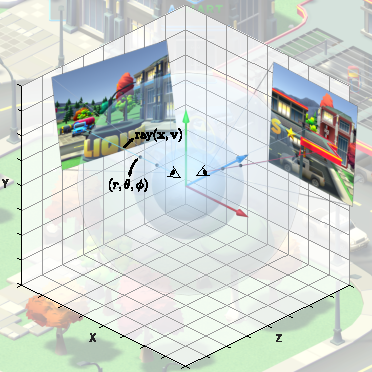
\includegraphics[width=0.96\linewidth]{TOG/figs/spher_coord.pdf}
%%    \caption{Visualization of our multi-spherical coordinate system.}
    \label{fig:method:coordinate}
%\end{figure}
% different position (10cm working, 50cm not working),
% different rotation

\dnc{(Jan 11) Ray to spherical coord} For a sphere with radius $r$, the intersection of ray and sphere $\pt_r$ can be calculated by solving:

\begin{equation}
    \|\pt_r\|^2=\|\rayo + k\rayd\|^2=r^2
\end{equation}

Convert $\pt_r$ to spherical coordinate $(r, \theta, \phi)$:

\begin{equation}
    \begin{cases}
        \theta = \mathrm{atan2}(x_{\pt_r}/z_{\pt_r})\\
        \phi = \mathrm{acos}(y_{\pt_r} / r)
    \end{cases}
\end{equation}

\dnc{(Jan 11) A simple derivation for the requirement of depth range and samples} Take 2D as an example. Consider two view centers $\rayo_1$, $\rayo_2$ on X axis and a point $\pt$ in 3D space. The radius of nearest sampling sphere of $\pt$ is $r_l$. The intersections of the sphere and rays from $\rayo_1$, $\rayo_2$ to $\pt$ are $\pt'_{1,r_l}$ and $\pt'_{2,r_l}$, respectively. $\Delta\pt'_{r_l}=\|\pt'_{2,r_l}-\pt'_{1,r_l}\|$ is small enough, then we have:

\begin{equation}
    \Delta\pt'_{r_l} \approx \Delta\rayo \frac{|z_\pt - r_l|}{z_\pt}
\end{equation}

\begin{equation}
    hello
\end{equation}

\begin{figure}[htb]
    \centering
    \includegraphics[width=0.96\linewidth]{TOG/figs/depth_disparity.pdf}
    \caption{Depth disparity}
    \label{fig:method:eccentricity}
\end{figure}

With this coordinate system, the input of individual element in the 3D spaces is defined as $p=(r, \theta, \phi)$ and the output is color information $c=(r,g,b)$ and volume density $d$. We train the scene representation with an multilayer perception (MLP) network first. 
For the training uniformity and run-time efficiency, we do not distinguish different eccentricities during the training stage. Instead, the spatially variant visual acuity is represented as varying field of views in the rendering, i.e., data creation.
Specifically, we depict the whole visual field as three semantic layers the fovea ({0-10 deg}), mid-periphery {6-60 deg}, and far periphery {y-110 deg}. In each frame, The uniformized networks returns three images with a identical resolution yet, as seen from the separation range in deg, gradually larger areas along eccentricity.

\begin{figure}[htb]
    \centering
    \includegraphics[width=0.96\linewidth]{TOG/figs/layers_together_zh.pdf}% try not overlapping the text on the image since we want the reviewers to see each pixel clearly
    \caption{Visualization of the output at three eccentricity ranges.}
    \label{fig:method:eccentricity}
\end{figure}

%estimate the fovea, mid-peripheral, peripheral field of view for a novel view next, fine-tune the fovea result with local view streamed from the cloud, and lastly warp/blend the three results for VR display.

\paragraph{Input encoding}
Since the input of our representation network is only three dimensional, we map the inputs to a higher dimensional space via high-frequency functions. \qisun{(Jan 9, 2021) What is bad if we have low-dim input? Harder to converge, higher error etc.?} \zh{(Jan 9) similar to NeRF, three components are not sufficient for achieving state-of-the-art quality, as demonstrated in Section 6.4). We introduce a positional encoding of the input coordinates that assists the MLP in
representing high-frequency functions.}
Thus we encoded the input through function:
\begin{align}
\iota (p) = (\sin(2^0 p), \cos(2^0 p), ..., \sin(2^{L-1}p, \cos(2^{L-1}p))
\label{eqn:inputencode}
\end{align}
The function $\iota (\cdot)$ is applied to each of the 3D location representation ($r$, $\theta$, and $\phi$), we choose $L$ to be 10 in practice. Hence, the input dimension becomes 3 x 20 = 60 after encoding. The MLP network is composed with $N_{layer}$ fully-connected layers, each uses ReLu as activation function and $N_{channel}$ channels per layer and output the color and volume density.

\paragraph{Synthesis}
% the description of the volume density is the same as chapter 4 in NeRF paper.
Similar to \cite{mildenhall2020nerf}, the trained representation is then deployed to synethesis final images via ray marching. For accelerating the performance, we bounded the near/far range to $20$ and $50$ meters respectively. The bounding, however, may introduce subtle quality drop, as shown in \Cref{fig:method:bounding}.
\begin{figure}
    \centering
    \subfloat[w bounding]{\includegraphics[width = 0.47\linewidth]{TOG/figs/depth_without_bound.png}}\hspace{1em}
    \subfloat[w/o bounding]{\includegraphics[width = 0.47\linewidth]{TOG/figs/depth_with_bound.png}}
    \caption{Visualization of ray marching bounding.}
    \label{fig:method:bounding}
\end{figure}
%For each pixel, we perform a ray from the camera and accumulate all the intersection's color weighted by the density accordingly between near bound and far bound. In practice, we experimented with different far bound values: 20 (meters) and 50 (meters), the difference between output is minimal. (\note{add figure for comparison}). We also experimented with the sampling number ($N_{sample}$) for accumulation between near bound and far bound to balance time cost and effects. Hence, we have an output image for the camera perspective.
However, as a gaze-contingent method, the compromised quality would be unnoticeable in periphery. Thus, we further refine the visual quality in foveal vision, as detailed in \Cref{sec:method:refine}.
Since we aim to render a novel view in real time and with perceptually high quality, we estimate the foveated image (10 degree), middle peripheral image (60 degree), and full peripheral image (110 degree) from the same novel view for further synthesis. Regarding foveated rendering, we estimate an image with size of 64 x 64, $N_{layer}=12$, $N_{channel}=64$, and $N_{sample}=16$. Regarding middle peripheral and full peripheral rendering, we estimate the two images with size of 256 x 256, $N_{layer}=8$, $N_{channel}=64$, and $N_{sample}=4$. We next upsample middle peripheral to ??? x ??? and full peripheral to 1440 x 1440 for blending.
\nothing{
\subsection{Refinement for Fovea Layer}
\label{sec:method:refine}
Due to the depth bounding and prediction errors, it is particularly challenging to preserve pixel-wise quality without compromising real-time performance. However, the human foveal vision is remarkably sensitive to subtle details across all frequency ranges. To 
To maximize the quality of foveated image, we utilize the limited but consistent network bandwidth by retrieving a local peripheral image from the cloud. The retrieval was realized by cloud-based rendering using users' upstreamed head and gaze parameters.
Due to the inevitable dual-way transmission, it is impossible to instantly obtain the image without latency. Displaying outdated frames have been studied as a major cause of simulator sickness.
}%nothing
\note{describe when to retrieve new full peripheral image.} We leverage local guidance views to fine tune the output foveated image. Local guidance view is decided according to current camera view. We chose the nearest 4 views (or 8 views) as reference views and estimate the color as well as volume density for all reference views. Every time we receive a new peripheral image from the cloud, we calculate the delta between the ground truth and our result for reference views for preparation. Then we warp the delta into target camera view, calculate the average and apply to the fovea result for each frame.

\subsection{Real-time Rendering}
% \subsection{Fovea-Peripheral Blending}
\label{sec:method:blending}
Lastly, we apply alpha blend on the fine-tuned fovea view and middle peripheral view, as well as on the middle peripheral view and full peripheral view via function smo/:

\subsection{Latency-quality joint optimization}
\label{sec:method:optimization}
Increasing rendering sampling naturally improves the image output quality. However, it increases the latency, causing quality drop stretched along time, and more critically, simulator sickness.
Inspired by \cite{Li:2020:TSP}, we perform a spatial-temporal joint optimization to determine the sampling that adapts to individual computational resources. This is achieved via a Pareto efficiency optimization. 

$E_{q}\triangleq $

$E_{l}$ is defined as the loss introduced by latency. 
\begin{align}
    \int E_{l} \mathbf{d} t
\end{align}

\begin{figure*}
    \centering
    \subfloat[quality-only]{\includegraphics[width=0.32\linewidth]{example-image-a}}
    \subfloat[latency-only]{\includegraphics[width=0.32\linewidth]{example-image-a}}
    \subfloat[ours]{\includegraphics[width=0.32\linewidth]{example-image-a}}
    \caption{Latency-quality joint-optimization.}
    \label{fig:optimization}
\end{figure*}

%\subsection{Cloud-Based System}
%\label{sec:method:system}
%Finally, we deploy our gaze-contingent synthesizer to a real-time cloud-based streaming system.
\section{Evaluation}
\label{sec:result}
% use one net to represent a complicated scene
% we still have other option for real-time, like streaming
\note{
Ablation studies for the network training/losses
Target scene | Foveated target scene | NeRF | network predicted images ---> at least 4 different scenes.
streaming time for 4-5 different scenes: full resolution vs our network prediction for “same data size”
image quality of rendered scene vs our network prediction for “same amount of streaming time”
User study results
Table on performance comparison, streaming time, PSNR, SSIM, etc
}%note
With a variety of scenes as shown in \Cref{fig:results:comparison2}, we evaluate our method with subjective studies (\Cref{sec:study:user}), objective analysis (\Cref{sec:study:quality}), and intra-system efficiency (\Cref{sec:study:intra}).
\begin{figure*}[htb]
    \centering
    \begin{minipage}{0.32\linewidth} %full res
        \subfloat[gas scene(\textbf{GT})]{\includegraphics[width=0.96\linewidth]{TOG/figs/gas_gt4.png}}
        
        \subfloat[minecraft scene(\textbf{GT})]{\includegraphics[width=0.96\linewidth]{TOG/figs/mc_gt3.png}}
        
        \subfloat[bedroom scene(\textbf{GT})]{\includegraphics[width=0.96\linewidth]{TOG/figs/bed_gt0.png}}
    \end{minipage}
    \begin{minipage}{0.32\linewidth} %ours
        \subfloat[gas scene (\textbf{OUR})]{\includegraphics[width=0.96\linewidth]{TOG/figs/gas_our4_inset.pdf}}
        
        \subfloat[minecraft scene (\textbf{OUR})]{\includegraphics[width=0.96\linewidth]{TOG/figs/mc_our3_inset.pdf}}
        
        \subfloat[bedroom scene (\textbf{OUR})]{\includegraphics[width=0.96\linewidth]{TOG/figs/bed_our0.png}}               
    \end{minipage}
    \begin{minipage}{0.32\linewidth} % NERF
        \subfloat[gas scene (\textbf{NeRF})]{\includegraphics[width=0.96\linewidth]{TOG/figs/gas_nerf4_inset.pdf}}
        
        \subfloat[minecraft scene (\textbf{NeRF})]{\includegraphics[width=0.96\linewidth]{TOG/figs/mc_nerf3_inset.pdf}}
        
        \subfloat[bedroom scene (\textbf{NeRF})]{\includegraphics[width=0.96\linewidth]{TOG/figs/bed_nerf0.png}}      
    \end{minipage}    
    
    \caption{Comparing our synthesis method (2nd column) with full resolution (1st column) rendering and NeRF (3rd column).}
    % {\zh{add inset for 2nd and 3rd col}}
    \label{fig:results:comparison}
\end{figure*}

\begin{figure*}[htb]
    \centering
    \begin{minipage}{0.32\linewidth} %full res
        
        \subfloat[gallery scene (\textbf{GT})]{\includegraphics[width=0.96\linewidth]{TOG/figs/gallery_GT_view_0001.png}}
    \end{minipage}
    \begin{minipage}{0.32\linewidth} %ours
        
        \subfloat[gallery scene (\textbf{OUR})]{\includegraphics[width=0.96\linewidth]{TOG/figs/gallery_our_001.png}}                
    \end{minipage}
    \begin{minipage}{0.32\linewidth} % NERF
        
        \subfloat[gallery scene (\textbf{NeRF})]{\includegraphics[width=0.96\linewidth]{TOG/figs/gallery_NeRF_001.png}}        
    \end{minipage}    
    
    \caption{Comparing our synthesis method (2nd column) with full resolution (1st column) rendering and NeRF (3rd column). (Cont.).}
    % {\zh{add inset for 2nd and 3rd col}}
    \label{fig:results:comparison2}
\end{figure*}

\subsection{User Study}
\label{sec:study:user}
% \zh{(Jan 10) all the Qs are answered offline, will update the section soon.}

% In this section, we report two perceptual experiments to investigate 1) how users perceive our solution and the ground truth and 2) how our solutions behaves compared to other alternatives.
We first conducted a perceptual experiment to investigate how users perceive our solution ({\bf OURS}) compared to existing solution (\cite{mildenhall2020nerf}, {\bf NeRF}) and original mesh with foveated rendering (\cite{perry2002gaze}, {\bf F-GT}).

% \zh{usually we report the study design here too, like within-subject user study and analyze method, like ANOVA. But I am not sure what we should use here.}
% \zh{(Jan 12), if we include NeRF, I'd say we keep one of the down-sample conditions}

\paragraph{Stimuli}

The stimuli were the images rendered via {\bf F-GT} or synthesized via  {\bf OURS}/{\bf NeRF}, as shown in \Cref{fig:results:comparison}. The resolution of the image per eye was $1440 \times 1600$. 
For fair comparison, each group of stimuli were generated with the same, randomly defined gaze p-osition. The position was indicated as a green cross on the stimuli images.
The resolution of the images per eye was $1440 \times 1600$. 
We used the {\it gas} and {\it minecraft} scenes.
Each condition from individual scene consists of $1$ view and $3$ different gaze positions.

Specifically, we controlled the foveal kernel size in {\bf F-GT} to match our display size and eye-display distances.
For generating {\bf NeRF} condition, we retrained the model from \cite{mildenhall2020nerf} on our dataset with $N_{sample}=16$, $N_{layers}=4$, $N_{channel}=128$. The last column of \Cref{fig:results:comparison} shows the result. 
%We predict the image from the camera transformation, fine-tune the foveated layer, and render the image by alpha blending the three layers.

%\zh{We probably don't need to attach foveated GT here}
% The second column is a uniformly down-sample image at size \warning{??? x ???}. Assuming our network bandwidth is \warning{???}, to stream the images from the cloud in real time, the largest size of the image per eye is up to \warning{??? = ??? / 50 fps / 2 eyes}. So we down sample the entire image with ratio \warning{???}.
%The second column enables foveated rendering. We applied \warning{foveated algorithms} described in \cite{perry2002gaze} and \cite{jiang2015salicon}. 
% and The foveated area is preserved as the original resolution while the rest of the image is down sampled. same alpha blending method that we used in our solution (see \autoref{sec:method:blending}). Similarly, we calculate the size of the foveated image based on the bandwidth. Hence the down-sample ratio of peripheral area is \warning{???}. 
%The third column is generated by NeRF implementation. We retrained a new model on our dataset with parameters $N_{sample}=16$, $N_{layers}=4$, $N_{channel}=128$. The last column is our result. We predict the image from the camera transformation, fine-tune the foveated layer, and render the image by alpha blending the three layers.

\paragraph{Setup}
Each participant was asked to wear a eye-tracked HTC Vive Pro Eye headset during the experiment. During the experiment, the participants wearing the headset examining  the stimuli. 
Fourteen users participated in the study and 13 of them managed to complete (4 females and 9 males, $M=23.08$, $SD=1.75$). One participant (age=23, female) did not complete the experiment due to gaze drifting (please refer to the task description below).
None of the subjects were aware of the research, the experimental hypothesis, or the number of rendering methods. All participants had normal or corrected-to-normal vision.

\paragraph{Task}
The task was a \textit{two-alternative-forced-choice} (2AFC). Each trial consists of a pair of stimuli from the three conditions ({\bf OURS} / {\bf NeRF} / {\bf F-GT}). Each stimulus appeared for $300$ms on the the display. A forced $1.5$sec break was introduced between conditions. During the study, the participants were instructed to fix their gazes on the green cross. To prevent fixation from shifting away, we tracked the users gaze during the whole experiment. Whenever the gaze is $1$deg away from the target, a trial was dropped immediately with black green informing the participant.
After each trial, the participants were instructed to select which one of the two stimuli appeared with higher visual quality using keyboard.
Before each experiment, a warm-up session with 1 trial was provided to have the participants familiarize the study procedure. The order of conditions cmong trials were randomized with counterbalancing.
%To start with, each participant was informed that they were required to choose an alternative with higher quality after watching each pair of stimuli. We calibrated the device and performed a warm-up trial to help participants understand our system. Each participant were provided with 1 warm-up trial and 6 official trials (2 scenes x 1 view x 3 gaze positions) where each trial consisted all the combinations of the pairs of every two stimuli. We randomize the order of the pairs for counterbalancing. We showed a yellow cross on the screen. After participants move their gaze positions to the area close to the cross, the yellow cross turns green. The first stimulus will be rendered as well as the cross after participants fixate the cross for 1 second. Each stimulus is displayed for 300 milliseconds. The second one will be rendered after 1.5-second dark screen. If the participants does not fixate at the cross when stimuli are displayed, the current pair will be discarded and displayed to the participants later in the same trial. After each pair, participants reported their opinions on which image has higher quality.
To minimize the effect of accumulating discomfort during the experiment, we enforced at least a 60-second break between each trial. Meanwhile, the participants were instructed to take as much time as needed to recover. 

\paragraph{Results}
\Cref{fig:results:2afc} plots the study results. 
Among all three conditions, we observed near to random guess among trails that compares  {\bf F-GT} and {\bf OURS} (50.0\% voted for {\bf OURS}). However, participants significantly prefers  {\bf F-GT} over {\bf NeRF} (98.7\% voted for NeRF, binomial test showed $p<0.005^{***}$). The preference applies to {\bf OURS} vs. {\bf F-GT} as well (97.4\% voted for NeRF, binomial test showed $p<0.005^{***}$).

% our/gt 78/156 0.5318897993488445
% our/nerf 152/156 2.6681140960754964e-40
% nerf/gt 2/156 1.3407579916082842e-43

\begin{figure}[htb]
    \centering
    \includegraphics[width=0.96\linewidth]{TOG/figs/vote.pdf}
    \caption{The users' preference votes from our evaluation experiment. X axis shows all the pair combination and Y axis shows the ratio of voting for the second one.}
    \label{fig:results:2afc}
\end{figure}

% apply binomial test https://docs.scipy.org/doc/scipy/reference/generated/scipy.stats.binom_test.html
% or apply ANOVA, there is a value of votes for each condition and we want to know if there exists significant effects on different condition.
\paragraph{Discussion}
The near-to-random-guess indicated the statistically similar perceptual quality between {\bf OURS} and foveated ground truth ({\bf F-GT}). 
Given the perceptual identicality between foveated and full-resolution rendering, the subjective study indicates that {\bf OURS} can achieve similar quality as a rendering with a locally fully stored high-quality mesh.
Meanwhile, both of the two conditions showed significant subjective quality preference than {\bf NeRF}. That is, under an immersive, high FoV, and first-person view, the current volume-based scene representation may not fully reproduce the perceptually identical retinal images.
To further validate the perceptual quality by breakdown across the whole visual field, we conducted measurements with objective metrics in the following section.

\subsection{Visual Quality}
\label{sec:study:quality}
Complementary to the subjective measurement (\Cref{sec:study:user}), we evaluate the perceived quality in an objective fashion. Specifically, under four different scenes (indoor/outdoor, artificial/realistic), we compare {\bf OURS}, {\bf F-GT} and {\bf NeRF} at individual eccentricity ranges across the whole visual field (up to $110$ deg, the capability of the VR HMD). 
%\zh{gonna comment this: To validate the non-uniform perceptual quality on the retina, we apply a foveated filtering to {\bf GT} \cite{perry2002gaze,jiang2015salicon}.}
For each eccentricity range, we compare the deep perceptual similarity (LPIPS) \cite{zhang2018unreasonable} across all scenes. LPIPS uses deep neural networks to evaluate perceptual similarity between the image provided and a reference image. Smaller values indicate higher perceptual similarity.
For each scene, we sample $20$ views with gazes at the middle of the display, resulting in $20$ data per eccentricity value, $420$ data per scene. We used one-way repeated measures ANOVAs to compare effects across three stimuli on each eccentricity value and together. Paired t-tests with Holm correction were used for all pairwise comparisons between stimuli. All tests for significance were made at the $\alpha=0.05$ level. 
% The error bars in the graphs show the 95\% confidence intervals of the means.

\paragraph{Results} 
\Cref{fig:lpips} plots LPIPS values across all scenes and eccentricity ranges ($5$ deg per sample). 
From foveal to near periphery (<=$40$ deg), we observed significant effects of the stimuli on LPIPS with a ``large'' effect size ($\eta^2 = 0.84$). That is, \textbf{OUR} shows significantly lower LPIPS than \textbf{NeRF} ($p<.001^{***}$), while significantly higher LPIPS than \textbf{F-GT} ($p<.001^{***}$).
For example, the main effects of stimuli ($F(2,38)=42.023, p=.001^{***}$) was significant on eccentricity $=25$  deg  in scene \textit{gas} (\Cref{fig:lpips:gas}). \textbf{OUR} was significantly lower than \textbf{NeRF} ($t(19)=-18.557, p<.001^{***}$) and \textbf{F-GT} ($t(19)=-10.342, p<.001^{***}$) both with a ``large'' effect size (Cohen's d $>0.8$). 

From mid- to far- periphery (>$40$ deg ), we observed significant effects of the stimuli on LPIPS with a ``large'' effect size ($\omega^2 = 0.19$). \textbf{OUR} shows significantly higher LPIPS than \textbf{NeRF} due to the foveated nature of our design. Whereas, comparing with \textbf{F-GT}, we observed  significant lower scores ($p<.001^{***}$).
For instance, the main effects of stimuli was significant on eccentricity $=60$ deg in scene \textit{gas} ($F(2,38)=493.51, p<.001^{***}$, \Cref{fig:lpips:gas}). \textbf{OUR} was significantly lower than \textbf{F-GT} ($t(19)=-12.28, p<.001^{***}$), and higher than \textbf{NeRF} ($t(19)=18.90, p<.001^{***}$) both with a ``large'' effect size (Cohen's d $>0.8$). 

The general trend applies to all 4 scenes being validated. 

\paragraph{Discussion}
The observation revealed our method's over-performance than alternative view synthesis solutions in the foveal and near peripheral vision. This is evidenced by the significantly increased perceptual similarity to \textbf{GT} while comparing between \textbf{OUR} and \textbf{NeRF}.\zh{``significantly increased LPIPS'' requires analysis}

Meanwhile, \textbf{OUR}'s increased perceptual similarity comparing with \textbf{F-GT} beyond $40$ deg indicated their similar visual quality. This shows that \textbf{OUR} doesn't compromise the peripheral vision's quality with its significantly enhanced foveal image. 

The discoveries also agrees with the trend from \Cref{sec:study:user}. That is, in addition to the faster performance, our method showed remarkably perceptual quality gain than \textbf{NeRF} for first-person 6DoF immersive viewing of 3D scenes: our synthesized views are perceptually identical to the traditionally rendered images from complete mesh. It yet achieves significant data storage saving (\warning{xxx\%-xxx\%}).

% ZH: why \Cref{fig:lpips:gas} shows 'section 5.2'
\begin{figure*}
    \centering
    \subfloat[gas]{\includegraphics[width=0.48\linewidth]{TOG/figs/lpips_scenegas.pdf}}\label{fig:lpips:gas}
    \subfloat[minecraft]{\includegraphics[width=0.48\linewidth]{TOG/figs/lpips_scenemc.pdf}}
    
    \subfloat[gallery]{\includegraphics[width=0.48\linewidth]{TOG/figs/lpips_scenegallery.pdf}}
    \subfloat[bedroom]{\includegraphics[width=0.48\linewidth]{TOG/figs/lpips_scenebedroom.pdf}}
    \caption{LPIPS analysis of all scenes as well as comparison of our method, NeRF, and foveated GT on each eccentricity.}
    {\zh{Add intersection lines later.}}
    \label{fig:lpips}
\end{figure*}

\subsection{Intra-System Workings}
\label{sec:study:intra}
\paragraph{Spatial-Temporal Optimality}

% apply objective metric to |cref{fig:optimization}, aka different sample numbers


\paragraph{Ablation Study}
% the performance of an AI system by removing certain components, to understand the contribution of the component to the overall system

% nmsl v.s. msl
\section{Conclusion}
\label{sec:conclusion}
In this paper, we present a gaze-aware neural scene representation and view synthesis method tailored for future portable virtual reality viewing experiences. Specifically, we overcome the limitations of existing neural rendering approaches for high performance, resolution, and fidelity. Our network individually synthesizes foveal, mid-, and far-periphery retinal images, which are then blended to form a wide field-of-view image matching retinal acuity. This is achieved via adapting the neural network model to the foveated visual acuity and stereopsis. 
Comparing with traditional rendering, our method requires less than $1\%$ data storage yet delivering identically high perceptual quality.
Comparing with alternative neural view synthesis approaches, our method creates significantly faster and higher fidelity viewing for high resolution, high FoV, and stereo VR head-mounted-displays.
%The experiments with user studies, objective measurements, and intra-system analysis show our significant effectiveness of delivering perceptually identical visual contents in real-time.
 
\paragraph{Limitations and future work}
While our method achieves unprecedented performance compared to existing approaches, it suffers from a few limitations. Our multi-spherical representation introduces higher quality when the VR camera is within the first sphere. As shown in \Cref{fig:large_translation}, when the virtual camera translates largely within a highly occluded scene, our method still synthesizes the accurate views but with declined foveal image quality. This is due to the accumulated error of the concentric spherical representation (\Cref{eq:imageError}).
Multiscale coordinates and networks that consider various level-of-details of the 3D space have shown their effectiveness of interpolating geometries \cite{winkler2010multi}. Developing a multiscale network that synthesizes the image from global to local level-of-details would be an interesting direction for future work, extending the applicability of our method to large-scale scenes with strong occlusions.
\begin{figure}[!ht]
    \centering
    % \subfloat[small translation]{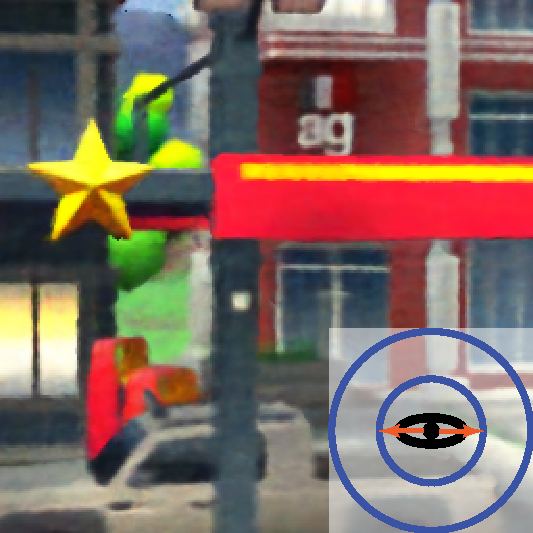
\includegraphics[width=0.47\linewidth]{TOG/figs/large_tran/2_gas_0.3.pdf}\label{fig:large_translation:small}}\hspace{1em} % or 2_gas_0.3.png
    \subfloat[small translation]{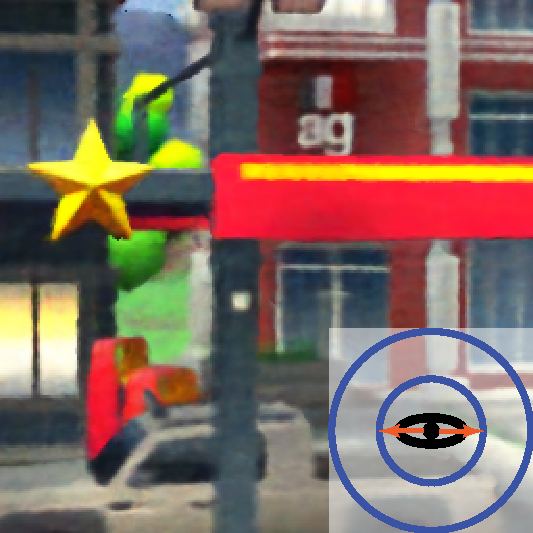
\includegraphics[width=0.47\linewidth]{TOG/figs/large_tran/2_gas_0.3.png}\label{fig:large_translation:small}}\hspace{1em}
    % \subfloat[large translation]{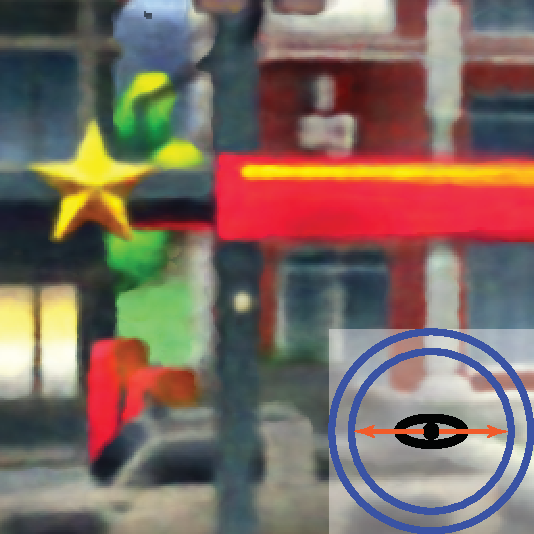
\includegraphics[width=0.47\linewidth]{TOG/figs/large_tran/2_gas_0.9.pdf}\label{fig:large_translation:large}} % or 2_gas_0.9.png
    \subfloat[large translation]{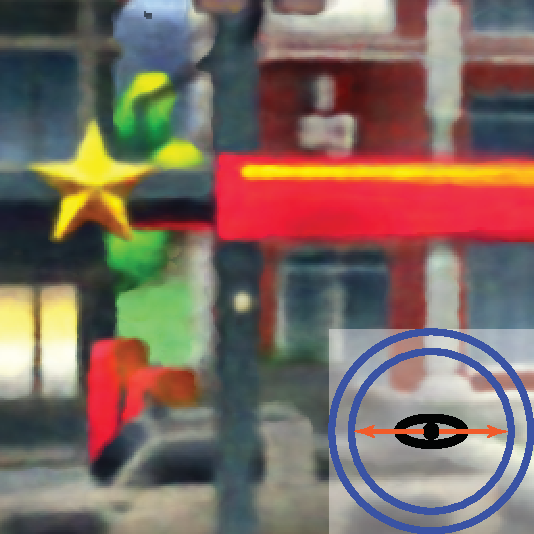
\includegraphics[width=0.47\linewidth]{TOG/figs/large_tran/2_gas_0.9.png}\label{fig:large_translation:large}}
    \Caption{Comparing foveal quality with regards to translation range. }
    {%
    Using our method, \subref{fig:large_translation:small} shows a fovea image \dnc{from training dataset} with a small-scale translation box (0.3m); \subref{fig:large_translation:large} shows a fovea image with a large-scale translation box (0.9m).
    }
    \label{fig:large_translation}
\end{figure}

Currently, we sample the scene fully based on eccentricity, considering acuity and stereopsis. However, we envision that fine-grained visual sensitivity analysis, such as luminance \cite{Tursun:2019:LCA} or depth \cite{Sun:20:OE}, would provide more insights on achieving even higher quality and/or faster performance. Also, our multi-spherical representation is specialized to the scene for optimal quality. Thus, our network is trained per-scene. Exploring potential means of generalized representation may further reduce storage.

For simplicity, the spatial-temporal joint optimization in \Cref{sec:method:optimization} connects the output precision and latency to the number of the spheres ($\sphereNum$) but not their radii $\mathbf{\sphereRadius}$. This is due to the significant amount of training with parameter sampling. Incorporating the parameters into a single training process may significantly reduce the time consumption for the optimization. With the adaptive training process, a content-aware distribution (i.e., $\mathbf{\sphereRadius}$) of the spheres would further improve the synthesis quality and performance.
%\qisun{note to myself: Right now we use did not optimize for radii but only number of spheres}

\zh{shall we end with non-limitation sentences?}\qisun{yep, future work is positive than limitations.;)}

\end{document}
